\documentclass{article}
\usepackage[margin=1.25in]{geometry}
\usepackage{amsmath, amssymb, setspace, enumerate, enumitem}
\usepackage{setspace}
\usepackage{graphicx}

\begin{document}
    \begin{enumerate}
        \item For any graph $G = (V,E)$, we can use an adjacency list to model it. By using depth first search, we can go through the entire graph. A sample algorithm would be to call DFS for each node, then you would look at all the nodes adjancent to that node, if they aren't marked (you can do a 1, 0 to mark them), then the algorithm would mark that node with the opposite of what your value is (if you are 0, then your adjancent node will be 1). If the algorithm completed the DFS algorithms and returns without an adjancent node being marked the same value as itself, then it is a bipartite graph.\\
        This achieves the $O(|V| + |E|)$ runtime because in DFS, we go through each node, and for each node, we go through all the edges for that node. In the end, we go through all the vertices and all the edges, therefore achieving this total runtime.
        \item Answer the following questions:
        \begin{enumerate}
            \item A DAG is a direct graph with no cycles. In a graph without any cycles, there must exist a node no indegree. Therefore, there is a source in any non-empty DAG.
            \item In an adjacency matrix, we can consider whether a node $i$ is connected with a node $j$ depending on whether or not the value of $A_{ij} = 0,1$. If it is 1, then node $i$ is connected to node $j$. To find it, we would have to traverse through all the nodes, and within each node, we have to check whether or not its connected with all other nodes. We will traverse through the entire matrix, and determine a source node if there exist a node with the value $0$ for any $i$ connected to it. Since we must traverse the entire matrix, the total runtime will the $O(|V|^2)$, or $\boxed{\mathbf{O(n^2)}}$. Below is a visualization of the algorithm.
            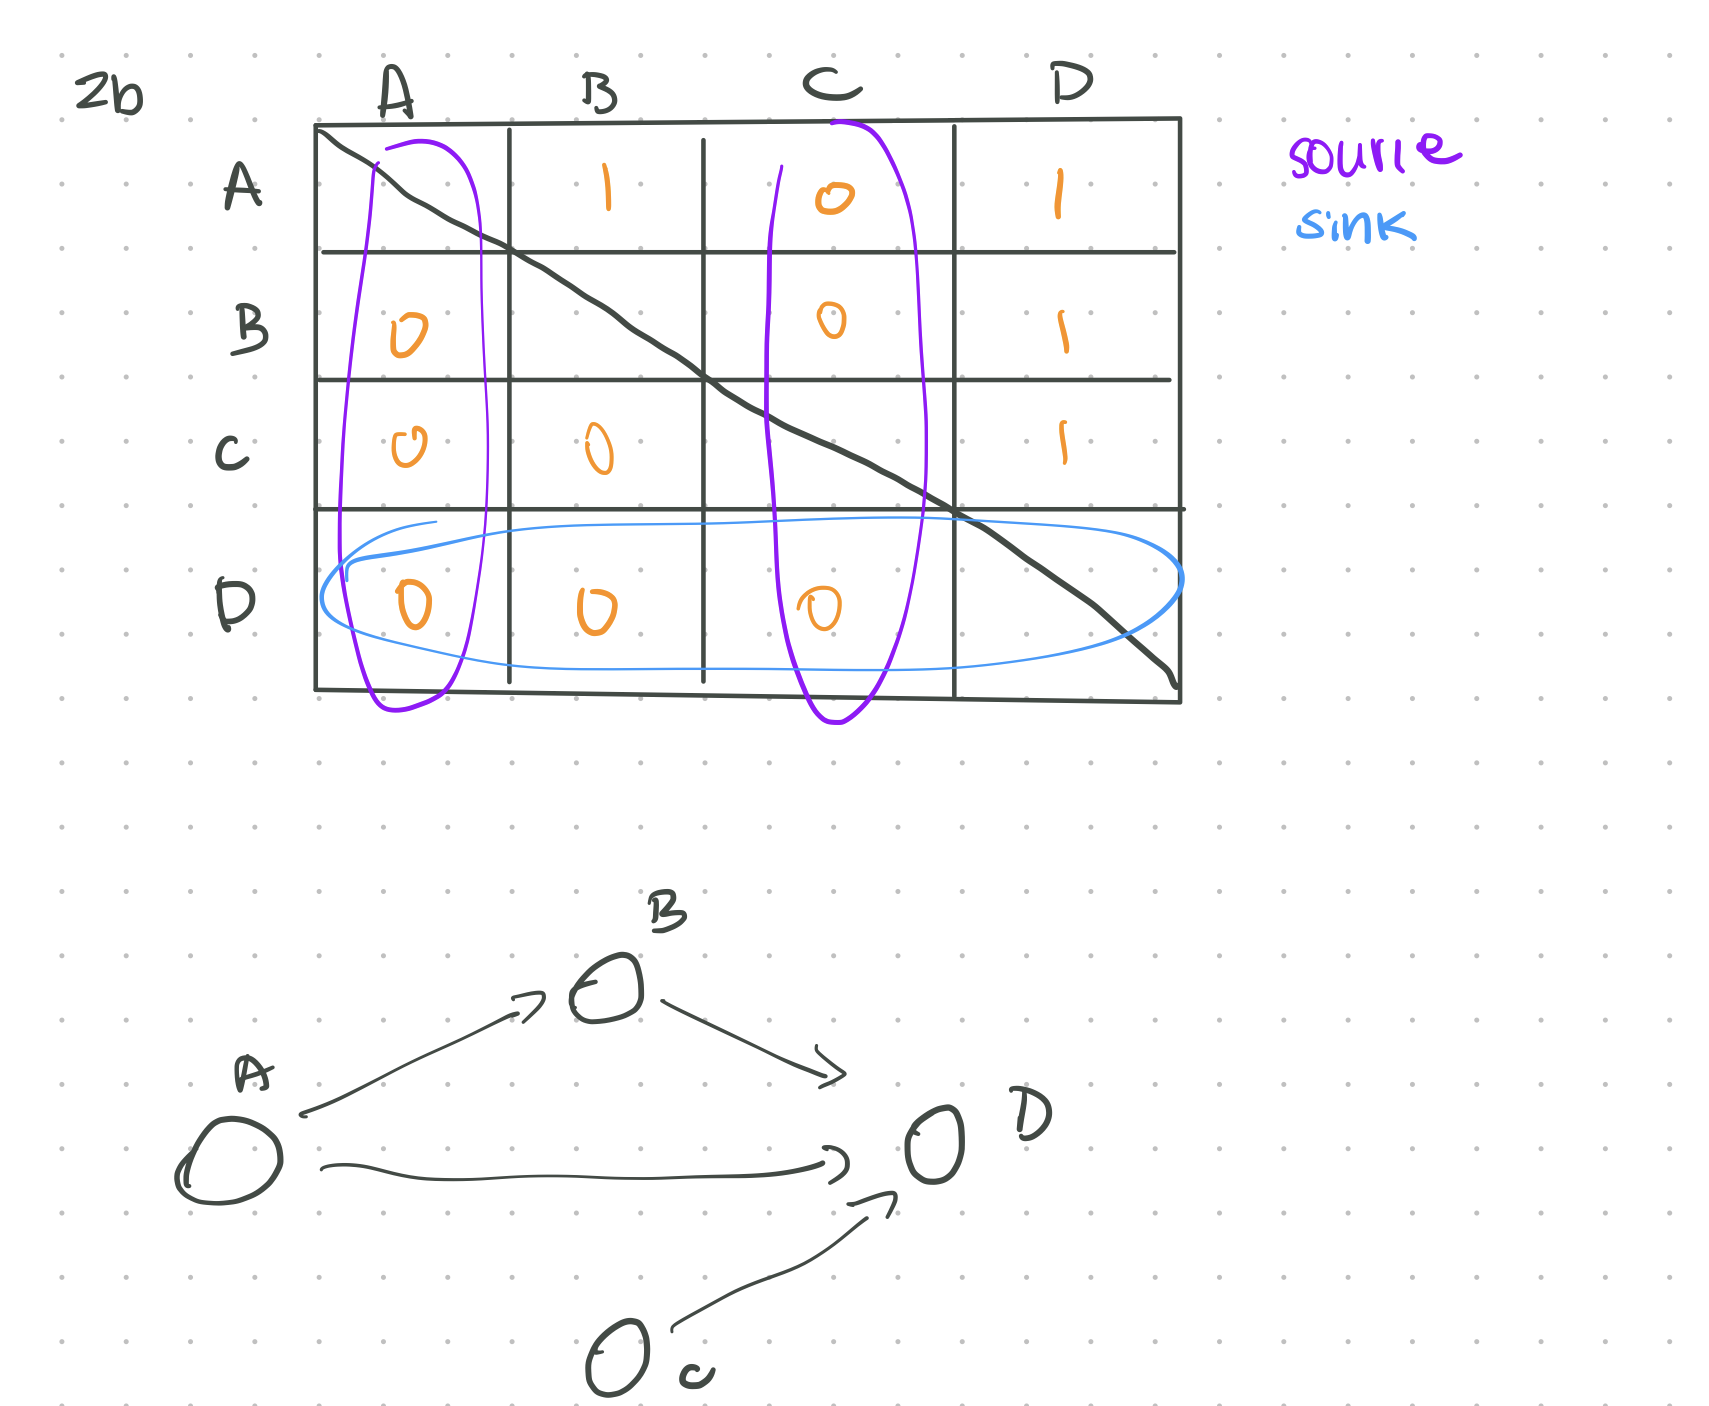
\includegraphics[scale=0.35]{2b.png}
            \item Here, we must go through all the nodes as well. If a node is a source node, it cannot appear in any linked list belonging to any of the $n$ nodes, therefore we have to check all the edges as well. This will equal to $O(|V| + |E|)$, or $\boxed{\mathbf{O(n + m)}}$. Below is a visualization of the algorithm.\\
            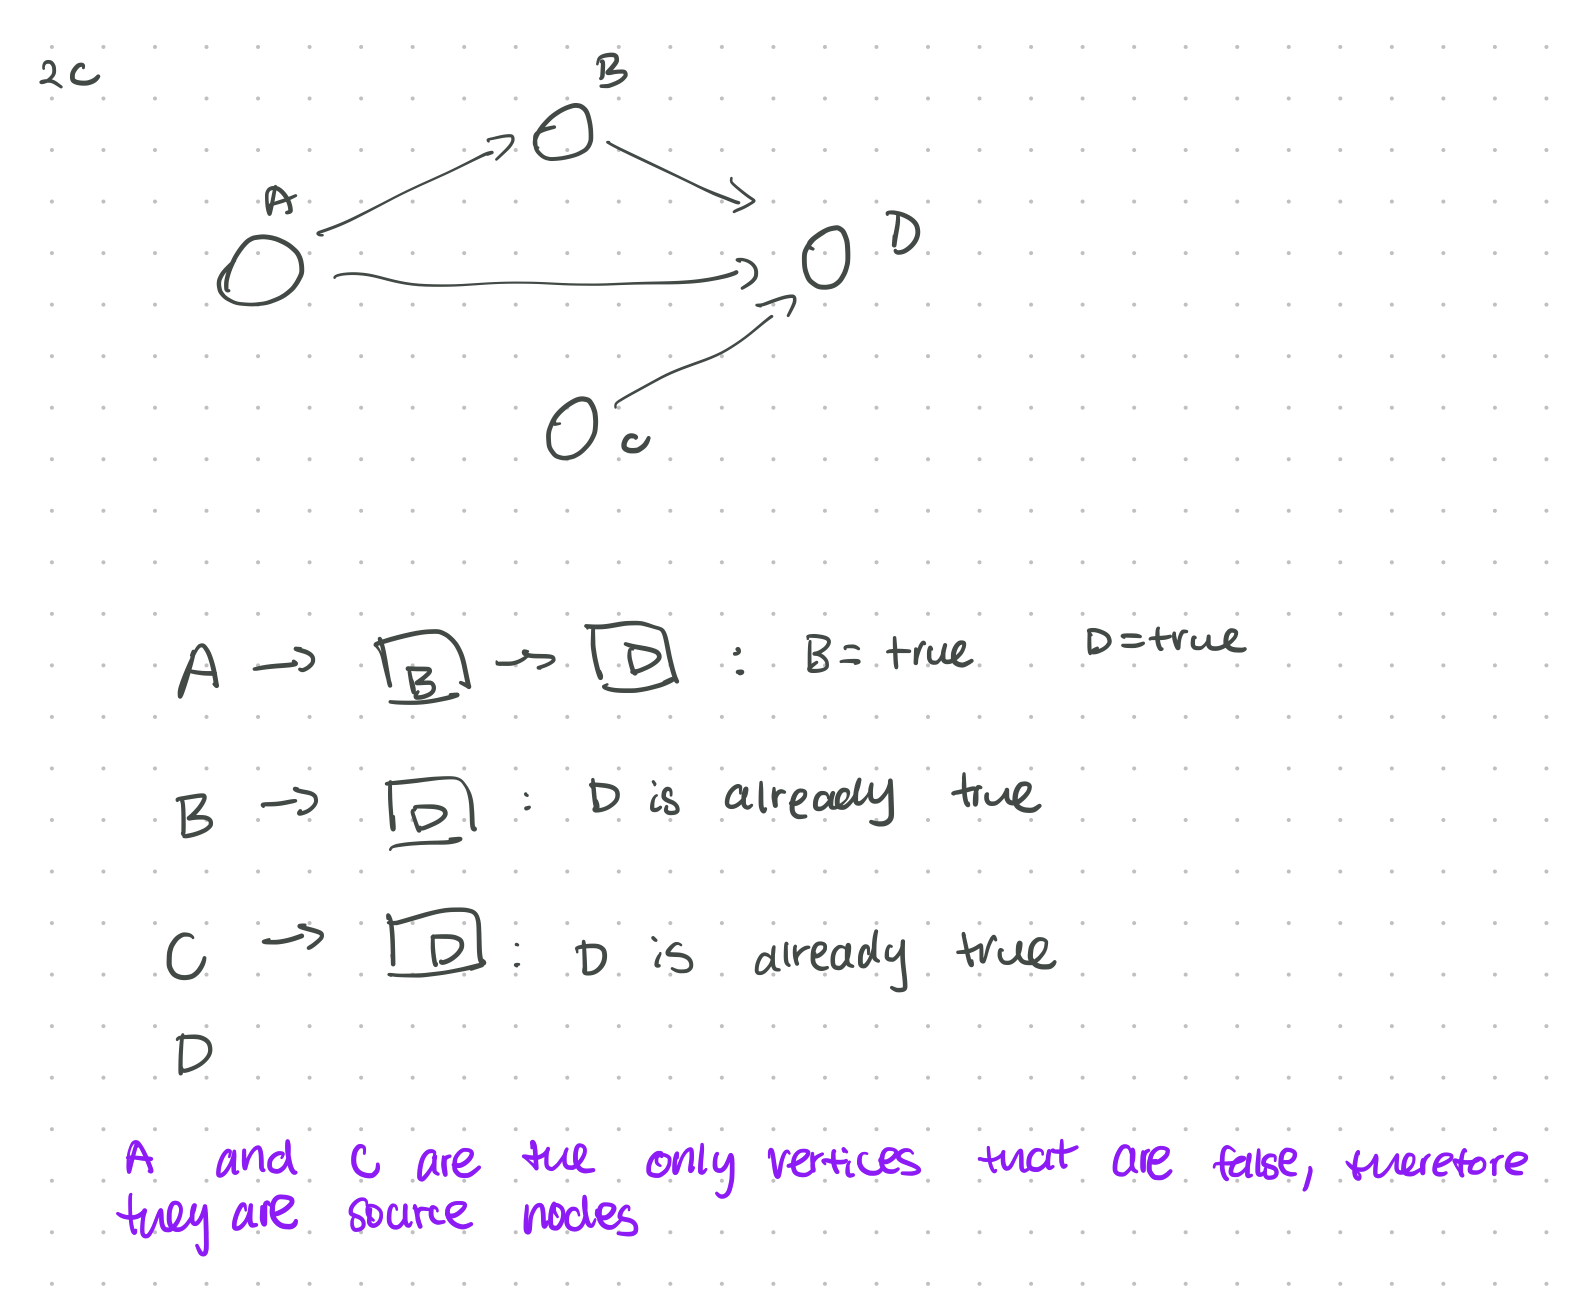
\includegraphics[scale=0.35]{2c.png}
        \end{enumerate}
    \end{enumerate}
\end{document}